\documentclass[11pt]{article}
\usepackage[final]{acl}
\usepackage{times}
\usepackage{latexsym}
\usepackage[T1]{fontenc}
\usepackage[utf8]{inputenc}
\usepackage{microtype}
% \usepackage{inconsolata}
\usepackage{graphicx}
\usepackage{amsmath}
\usepackage{booktabs}
\usepackage{hyperref}
\usepackage{xcolor}
\usepackage{tikz}
\usetikzlibrary{shapes.geometric, arrows.meta, positioning}

% Compress spacing
\usepackage{setspace}
\setlength{\parskip}{0pt}
\setlength{\floatsep}{4pt}
\setlength{\textfloatsep}{6pt}
\setlength{\intextsep}{4pt}

\hypersetup{
  colorlinks=true,
  linkcolor=blue,
  citecolor=blue,
  urlcolor=blue
}

% Tighten spacing to fit content within 4 pages before references
\usepackage{setspace}
\setlength{\parskip}{0pt}
\setlength{\floatsep}{4pt plus 1pt minus 1pt}
\setlength{\textfloatsep}{6pt plus 1pt minus 1pt}
\setlength{\intextsep}{4pt plus 1pt minus 1pt}
\setlength{\abovecaptionskip}{3pt}
\setlength{\belowcaptionskip}{1pt}

\title{PrimeLine@DravidianLangTech 2026: Hope Speech Detection in Tulu\\
Using XLM-RoBERTa for Coarse and Fine-Grained Classification}

\author{
  \textbf{Rithikaa V} \quad \textbf{Sanjay Krishnan K} \quad \textbf{Nithya Varshini C N R} \quad \textbf{S. Sumathi}\\
  Department of Information Technology, St.\ Joseph's College of Engineering\\
  \href{https://github.com/Rithikaa7/PrimeLine-Hope_Speech_Detection}{\texttt{https://github.com/Rithikaa7/PrimeLine-Hope\_Speech\_Detection}}
}

\begin{document}
\maketitle

\begin{abstract}
Hope speech detection in low-resource, code-mixed languages presents a genuine challenge
for natural language processing. Tulu, a Dravidian language spoken along the coastal regions of Karnataka and Kerala, is one such
language where social media content is deeply
code-mixed, blending Tulu, Kannada script,
and English within a single comment. Two
classification tasks are addressed: a four-class
coarse-grained setting (Track~1) and a five-class
fine-grained setting (Track~2). XLM-RoBERTa,
a cross-lingual transformer pre-trained on more
than 100 languages, is fine-tuned on the task-provided datasets using Google Colab with
an NVIDIA T4 GPU. The system achieves a
Macro F1-score of 0.34 on Track~1 and 0.19
on Track~2 on the official Codabench evaluation, establishing the first transformer-based
baseline for hope speech classification in Tulu.
\end{abstract}

\section{Introduction}

Hope speech refers to positive, forward-looking online content that encourages, supports, or inspires
others. As NLP research has expanded its scope,
hope speech detection has grown into a meaningful
area of study, offering a constructive counterpart
to the widely explored tasks of hate speech and
toxicity detection. While considerable effort has
been directed at identifying harmful content, the
computational identification of positive and hopeful discourse has received comparatively less attention.

Identifying hopeful language in regional and
minority languages is particularly valuable, as it
gives visibility to communities rarely represented
in large-scale language studies. For speakers of
languages such as Tulu, computational tools can
open up possibilities for social listening and content moderation tailored to their specific needs.

Tulu is spoken by roughly four to five million
people in the Tulu Nadu region of coastal Karnataka and Kerala. Despite its significant speaker
population, Tulu remains almost entirely absent
from NLP research. There is no dedicated pre-trained language model for Tulu and no established
NLP pipeline for the language. Its presence on social media is marked by heavy code-mixing, where
native Tulu, Kannada script, English, and emoji are
blended freely within a single comment, making
automated classification considerably harder than
equivalent tasks in monolingual settings.

The DravidianLangTech shared task on Hope
Speech Detection in Tulu, organized as part of ACL
2026, provides the first structured benchmark for
this problem. Track~1 covers four coarse-grained
categories: Encouraging Hope, Discouraging Hope,
Blended Hope, and Uninvolved. Track~2 covers five
fine-grained categories: Inspiring Hope, Hopelessness, Realistic Hope, Optimistic Hope, and Fading
Hope. The transition to fine-grained classification
makes the task progressively more demanding, as
Track~2 categories differ in degree rather than in
kind, with genuinely ambiguous boundaries.

The approach taken in this work centers on fine-tuning XLM-RoBERTa \cite{conneau2020}, a multilingual transformer pre-trained on more than 100 languages.
Its cross-lingual representations allow it to handle
Tulu's mixed scripts without any language identification or transliteration steps, making it a practical
and principled choice for this low-resource, code-mixed setting. The system is trained end-to-end
with a linear classification head on top of the encoder, and predictions are generated by taking the
argmax of the softmax output.

\section{Related Work}

Hope speech detection as a formal NLP task was
first introduced by \citet{chakravarthi2020} through the
HopeEDI dataset, covering English, Tamil, and
Malayalam. The dataset and baselines demonstrated that transformer-based models clearly outperform classical approaches even on small multilingual corpora, setting the stage for the shared
tasks that followed.

\citet{chakravarthi2021findings} reported findings from a shared task on hope speech detection
across English, Tamil, and Malayalam, confirming that multilingual transformers consistently outperform classical machine learning approaches on
code-mixed text.

Several systems from those shared tasks demonstrated the strength of XLM-RoBERTa. \citet{ziehe2021} showed that fine-tuning XLM-RoBERTa
achieved strong results across English, Malayalam,
and Tamil without any task-specific feature engineering. \citet{mahajan2021} ranked first in both English and Tamil by fine-tuning RoBERTa and XLM-RoBERTa respectively. \citet{balouchzahi2021} built
an XLM-RoBERTa ensemble specifically for code-mixed Dravidian text. \citet{huang2021} combined
XLM-RoBERTa with TF-IDF features and ranked
first in both English and Malayalam. \citet{singh2021} explored multilingual transformer models pre-trained on Indian languages and achieved second
place in both English and Malayalam. These results collectively established XLM-RoBERTa as
the dominant baseline for Dravidian hope speech
classification.

On the model side, \citet{vaswani2017} introduced the Transformer architecture, which set the
foundation for the modern pre-trained language
model paradigm. \citet{devlin2019} built on this
with BERT, demonstrating the power of masked
language modelling for downstream NLP tasks.
\citet{liu2019} followed with RoBERTa, showing
that more robust pre-training strategies yield better
performance. \citet{conneau2020} extended this to
the multilingual setting with XLM-RoBERTa, pre-trained on over 100 languages including several
Indic scripts.

Dravidian language NLP has received growing
attention in recent years. \citet{chakravarthi2022overview} reported a comprehensive shared task overview on
hope speech across five languages. \citet{chakravarthi2022multilingual} further presented a multilingual hope speech
dataset covering English and Dravidian languages.
\citet{sundar2022} proposed a stacked encoder architecture using cross-lingual embeddings and demonstrated improvements over standard fine-tuning
baselines.

Research on Tulu specifically is extremely
sparse. \citet{shetty2023} examined sentiment analysis in
code-mixed Tulu and Tamil text, noting the severe
scarcity of annotated data. \citet{ehsan2023} tackled
Tulu sentiment classification using BiLSTM models with ELMo embeddings, identifying the lack
of Tulu-specific language resources as the primary
bottleneck. Neither work addresses hope speech
detection in Tulu; the current work is the first to do
so.

\section{Dataset and Preprocessing}

\subsection{Dataset}

The datasets for both tracks were prepared by the
shared task organizers and drawn from social media platforms used by Tulu speakers. The text reflects real-world Tulu online writing, mixing Tulu,
Kannada script, English, and emoji freely within individual comments. This code-mixed, multi-script
nature is a defining feature of the data and makes
classification non-trivial even for human annotators.

Track~1 contains 5,991 training samples across
four coarse categories. The distribution is imbalanced, with Uninvolved accounting for 2,490 samples (41.6\%) and Discouraging Hope having the
fewest at 711 (11.9\%). Track~2 has 3,185 training
samples across five fine-grained labels, with Inspiring Hope as the majority class at 35.4\% and Fading
Hope as the minority at 7.4\%. Tables~\ref{tab:track1} and \ref{tab:track2} show
the full distributions.

\begin{table}[h]
\centering
\begin{tabular}{lrr}
\toprule
\textbf{Label} & \textbf{Count} & \textbf{\%} \\
\midrule
Encouraging Hope & 1895 & 31.6\% \\
Discouraging Hope & 711 & 11.9\% \\
Blended Hope & 895 & 14.9\% \\
Uninvolved & 2490 & 41.6\% \\
\midrule
Total & 5991 & 100\% \\
\bottomrule
\end{tabular}
\caption{Class distribution -- Track~1 (Coarse-Grained).}
\label{tab:track1}
\end{table}

\begin{table}[h]
\centering
\begin{tabular}{lrr}
\toprule
\textbf{Label} & \textbf{Count} & \textbf{\%} \\
\midrule
Inspiring Hope & 1129 & 35.4\% \\
Hopelessness & 937 & 29.4\% \\
Realistic Hope & 503 & 15.8\% \\
Optimistic Hope & 380 & 11.9\% \\
Fading Hope & 236 & 7.4\% \\
\midrule
Total & 3185 & 100\% \\
\bottomrule
\end{tabular}
\caption{Class distribution -- Track~2 (Fine-Grained).}
\label{tab:track2}
\end{table}

\subsection{Preprocessing}

Preprocessing was kept minimal by design. Text
samples were passed directly to the XLM-RoBERTa tokenizer, which handles diverse scripts
through a SentencePiece-based subword vocabulary. Padding and truncation were applied at a maximum length of 128 tokens. Transliteration, language identification, and stopword removal were
deliberately skipped, as these steps risk erasing
code-switching cues that carry genuine meaning.
No normalization of Kannada or Roman script was
applied, preserving the natural variation present
in user-generated content. This minimal preprocessing strategy is consistent with prior work on
code-mixed Dravidian NLP, where aggressive preprocessing has been shown to hurt rather than help
performance.

\section{Methodology}

\subsection{System Pipeline}

The system follows a standard transformer fine-tuning pipeline. Each raw text sample is first passed
to the XLM-RoBERTa tokenizer, which applies
SentencePiece subword segmentation and encodes
the input as a sequence of token IDs with a special
\texttt{[CLS]} token prepended. The encoded sequence
is fed into the XLM-RoBERTa encoder, which
produces contextualized representations through
twelve layers of multi-headed self-attention. The
hidden state of the \texttt{[CLS]} token at the final encoder layer is extracted and passed through a linear
classification head. Output logits are converted to
class probabilities via softmax, and the predicted
label is the class with the highest probability. For
Track~1, the output layer has four neurons; for
Track~2, five. Figure~\ref{fig:pipeline} illustrates the pipeline.

\begin{figure}[h]
\centering
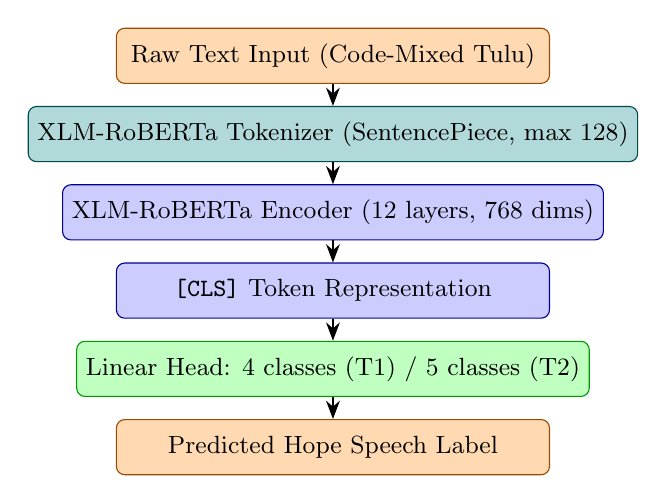
\begin{tikzpicture}[
  node distance=0.28cm,
  box/.style={rectangle, rounded corners=3pt, draw, text centered, minimum height=0.7cm, minimum width=5.5cm, font=\small},
  orangebox/.style={box, fill=orange!30, draw=orange!60!black},
  tealbox/.style={box, fill=teal!30, draw=teal!60!black},
  bluebox/.style={box, fill=blue!20, draw=blue!60!black},
  greenbox/.style={box, fill=green!25, draw=green!60!black},
  arr/.style={-Stealth, thick}
]
\node[orangebox] (input) {Raw Text Input (Code-Mixed Tulu)};
\node[tealbox, below=of input] (tok) {XLM-RoBERTa Tokenizer (SentencePiece, max 128)};
\node[bluebox, below=of tok] (enc) {XLM-RoBERTa Encoder (12 layers, 768 dims)};
\node[bluebox, below=of enc] (cls) {\texttt{[CLS]} Token Representation};
\node[greenbox, below=of cls] (head) {Linear Head: 4 classes (T1) / 5 classes (T2)};
\node[orangebox, below=of head] (out) {Predicted Hope Speech Label};

\draw[arr] (input) -- (tok);
\draw[arr] (tok) -- (enc);
\draw[arr] (enc) -- (cls);
\draw[arr] (cls) -- (head);
\draw[arr] (head) -- (out);
\end{tikzpicture}
\caption{End-to-end system pipeline for hope speech classification in Tulu.}
\label{fig:pipeline}
\end{figure}

\subsection{Model Formulation}

The core of the system is \texttt{xlm-roberta-base},
a transformer encoder built on the architecture of
\citet{vaswani2017} and trained using the robust
pre-training strategy of \citet{liu2019} extended to
100+ languages by \citet{conneau2020}. The model
contains approximately 270 million parameters and
was pre-trained on filtered Common Crawl data
spanning 100 languages, including Indic scripts.

Within each transformer layer, the self-attention
mechanism computes attention scores over all token pairs. Given query matrix $\mathbf{Q}$, key matrix $\mathbf{K}$,
and value matrix $\mathbf{V}$, scaled dot-product attention
is:
\begin{equation}
\text{Attention}(\mathbf{Q}, \mathbf{K}, \mathbf{V}) = \text{softmax}\!\left(\frac{\mathbf{Q}\mathbf{K}^\top}{\sqrt{d_k}}\right)\mathbf{V}
\end{equation}
where $d_k$ is the key vector dimensionality. This allows the model to capture long-range dependencies
across mixed scripts and languages simultaneously.

The \texttt{[CLS]} representation is fed into a linear
head, and logits $z_1, \ldots, z_C$ are normalized via softmax to produce class probabilities:
\begin{equation}
P(y = c \mid x) = \frac{\exp(z_c)}{\sum_{j=1}^{C} \exp(z_j)}
\end{equation}

The model is trained end-to-end by minimizing
categorical cross-entropy loss:
\begin{equation}
\mathcal{L} = -\frac{1}{N}\sum_{i=1}^{N}\sum_{c=1}^{C} y_{ic} \log P(y = c \mid x_i)
\end{equation}
where $N$ is the number of training samples, $C$
the number of classes, and $y_{ic} \in \{0,1\}$ the one-hot ground truth indicator. Gradients are backpropagated through the full encoder, adapting pre-trained representations to the specific vocabulary
and style of Tulu social media text.

\subsection{Training Setup}

Both models were fine-tuned on Google Colab with
an NVIDIA T4 GPU for 2 epochs with batch size 8
and AdamW optimizer (learning rate $2\times10^{-5}$,
weight decay 0.01). A linear warmup was applied
over the first 6\% of training steps, followed by linear decay to zero. The development set served as
the validation split throughout, and the best checkpoint by validation loss was selected for inference.
Predictions on test sets were obtained by argmax
over output logits, converted to label strings, and
submitted to Codabench. No ensembling was applied.

\section{Results and Discussion}

\subsection{Official Results}

Table~\ref{tab:results} reports official Codabench evaluation
scores. Accuracy and macro-averaged precision,
recall, and F1 are reported. Macro-averaging is
the primary metric as it weights all classes equally,
making it sensitive to performance on minority categories regardless of their frequency.

\begin{table}[h]
\centering
\begin{tabular}{lcccc}
\toprule
\textbf{Track} & \textbf{Acc} & \textbf{P} & \textbf{R} & \textbf{F1} \\
\midrule
Track 1 -- Coarse & 0.60 & 0.30 & 0.41 & 0.34 \\
Track 2 -- Fine   & 0.24 & 0.19 & 0.19 & 0.19 \\
\bottomrule
\end{tabular}
\caption{Macro-averaged results on Codabench (P\,=\,Precision, R\,=\,Recall).}
\label{tab:results}
\end{table}

On Track~1, an accuracy of 0.60 is achieved with
a Macro F1 of 0.34. The gap between these two
figures reflects a model that performs well on the
majority Uninvolved class but struggles with less
frequent categories. Track~2 is harder, with accuracy at 0.24 and Macro F1 at 0.19, reflecting the semantic closeness of its five fine-grained categories
and severe class imbalance.

\subsection{Error Analysis}

A detailed look at predictions reveals that the
accuracy-F1 gap on Track~1 is driven primarily
by over-prediction of the Uninvolved class (41.6\%
of training data). Samples from Blended Hope and
Discouraging Hope are prone to being absorbed
into this dominant category, as they share surface-level vocabulary with neutral comments. The decision boundary between Encouraging Hope and
Blended Hope is especially difficult, since a comment can simultaneously express genuine positivity
and realistic acknowledgment of hardship, making
clean categorical assignment ambiguous.

Track~2 exhibits a more extreme version of the
same problem. The five fine-grained categories are
semantically adjacent and differ in degree rather
than kind. A comment expressing uncertainty
about the future could plausibly belong to Fading
Hope, Hopelessness, or Realistic Hope depending
on subtle contextual cues difficult to capture with
only two epochs of fine-tuning. The scarcity of
Fading Hope samples (236 of 3,185) further limits
learning for this class.

\subsection{Discussion and Future Directions}

The results demonstrate that XLM-RoBERTa provides a viable starting point for hope speech detection in Tulu even without Tulu-specific pre-training.
Future work should address class imbalance via
weighted loss functions or back-translation augmentation from Kannada. Training for more
epochs with early stopping based on macro F1
could help balance performance across classes.
Larger multilingual models or Dravidian-family-specific pre-trained models could yield better representations for Tulu's lexical patterns. Contrastive
learning objectives that explicitly separate semantically similar hope categories could also resolve
the fine-grained boundary confusion observed in
Track~2.

\vspace{-2pt}
\section{Conclusion}

This work presents the first transformer-based
system for hope speech detection in code-mixed
Tulu, fine-tuned on datasets from the DravidianLangTech@ACL 2026 shared task. XLM-RoBERTa is applied to both tracks, achieving
Macro F1 scores of 0.34 and 0.19 on Track~1
and Track~2 respectively. The results establish
a meaningful baseline for future work and highlight the dual challenge of class imbalance and
fine-grained semantic similarity. Despite modest
absolute scores, the cross-lingual transfer capabilities of XLM-RoBERTa prove sufficient to produce
non-trivial predictions even for a language with
no dedicated NLP resources. It is hoped that this
contribution encourages further computational research on Tulu and other low-resource Dravidian
languages that remain largely absent from the NLP
literature.

\vspace{-2pt}
\section*{Limitations}

The primary limitation is the use of only two training epochs, restricting the model's ability to learn
reliable decision boundaries for minority classes.
The absence of Tulu-specific pre-trained representations means cross-lingual transfer may not
fully capture the language's phonological and morphological patterns. Class imbalance was not addressed through resampling or loss-weighting, suppressing performance on rare categories. The system does not perform language identification or
script normalization, both avenues for future improvement.

\vspace{-2pt}
\section*{Acknowledgments}

The organizers of the DravidianLangTech@ACL 2026 shared task are thanked
for providing the datasets and the Codabench
evaluation platform. Sincere gratitude is expressed
to the project guide, S.~Sumathi, Department of
Information Technology, St.~Joseph's College of
Engineering, for constant guidance throughout this
work.

\setlength{\bibsep}{0pt}
\footnotesize
\bibliography{references}

\end{document}
